%%%%%%%%%%%%%%%%%%%%%%%%%%%%%%%%%%%%%%%%%
% Beamer Presentation
% LaTeX Template
% Version 1.0 (10/11/12)
%%%%%%%%%%%%%%%%%%%%%%%%%%%%%%%%%%%%%%%%%
%----------------------------------------------------------------------------------------
%    PACKAGES AND THEMES
%----------------------------------------------------------------------------------------
\documentclass[aspectratio=169]{beamer}
\mode<presentation> {
\usetheme{Madrid}
}

\usepackage{graphicx} % Allows including images
\usepackage{booktabs} % Allows the use of \toprule, \midrule and \bottomrule in tables
\usepackage{multicol}
\usepackage{multirow}
\usepackage{longtable}
\usepackage[utf8]{inputenc}
\usepackage{enumerate}
\usepackage{color,url}
% ########## user defined
\usepackage{tikz}
\usetikzlibrary{patterns}
\usepackage{calc}
\usepackage{subfig}
\usepackage{pgfplots}
\pgfplotsset{compat=1.9}
\usepackage{pgf-pie}
\usepackage{algorithm}
\usepackage{algpseudocode}
\usepackage{listings}
\lstset{language=Python,basicstyle=\ttfamily,keywordstyle=\color{blue}}
\usepackage{caption}

\AtBeginSection[]{
  \begin{frame}
  \vfill
  \centering
  \begin{beamercolorbox}[sep=8pt,center,shadow=true,rounded=true]{title}
    \usebeamerfont{title}\insertsectionhead\par%
  \end{beamercolorbox}
  \vfill
  \end{frame}
}

%----------------------------------------------------------------------------------------
%    TITLE PAGE
%----------------------------------------------------------------------------------------
\title{Leitura Quest}
\subtitle{Sistema de Informa\c{c}\~ao}

\author[Cau\^e Trindade, Pedro Cirqueira, Pedro Conti]{Cau\^e Trindade \newline Pedro Cirqueira \newline Pedro Conti}

\institute[UnB]{Universidade de Bras\'ilia (UnB) \\ 
    \medskip
    \date{August 25, 2022}}

\begin{document}

\begin{frame}
\titlepage
\end{frame}

\begin{frame}
\frametitle{Sum\'ario}
\tableofcontents
\end{frame}

\section{Visão Geral do Protótipo}

\begin{frame}{Objetivo do Recorte}
\begin{itemize}
    \item Apresentar o protótipo como evidência de aderência entre produto, requisitos e dados.
    \item Mostrar rastreabilidade entre telas, RFs, HUs e épicos usando o documento de relação protótipo-funcionalidades.
    \item Destacar como o desenho de dados sustenta leitura, gamificação, comunidade e acompanhamento pedagógico.
\end{itemize}

\vspace{0.2cm}
\textbf{Foco:} narrativa de produto orientada por evidências visuais do protótipo.
\end{frame}

\begin{frame}{Mapa de Jornadas no Protótipo}
\begin{columns}
\column{0.48\textwidth}
\textbf{Jornada 1: Acesso}
\begin{itemize}
    \item Login
    \item Cadastro em duas etapas
    \item Recupera\c{c}\~ao de senha
\end{itemize}

\textbf{Jornada 2: Leitura}
\begin{itemize}
    \item Home com biblioteca e busca
    \item Detalhe do livro
    \item Registro de progresso
\end{itemize}

\column{0.48\textwidth}
\textbf{Jornada 3: Gamifica\c{c}\~ao}
\begin{itemize}
    \item Loja e itens de avatar
    \item Pontos, moedas e ranking
\end{itemize}

\textbf{Jornada 4: Comunica\c{c}\~ao}
\begin{itemize}
    \item Comunidades
    \item Painel de desempenho
    \item Mural de avisos
\end{itemize}
\end{columns}
\end{frame}

\begin{frame}{Legenda de Épicos (identificação)}
\small
\begin{itemize}
    \item \textbf{EP001 -- ACC:} Autenticação e Acesso
    \item \textbf{EP002 -- PERF:} Perfil e Personalização
    \item \textbf{EP003 -- BIB:} Biblioteca e Leitura
    \item \textbf{EP004 -- GAME:} Gamificação e Rankings
    \item \textbf{EP005 -- COM:} Comunidades e Interação
    \item \textbf{EP006 -- PED:} Gestão Pedagógica
    \item \textbf{EP007 -- AVS:} Eventos e Avisos
\end{itemize}
\end{frame}

\begin{frame}{Legenda de Requisitos (identificação)}
\scriptsize
\begin{itemize}
    \item \textbf{RF001 -- CAD:} Cadastro de usuários
    \item \textbf{RF002 -- AUT:} Autenticação por login e senha
    \item \textbf{RF003 -- AVT:} Personalização de avatar
    \item \textbf{RF004 -- BIBD:} Biblioteca digital
    \item \textbf{RF005 -- DETL:} Detalhes de livros
    \item \textbf{RF006 -- PRG:} Registro de progresso de leitura
    \item \textbf{RF007 -- PONT:} Pontuação e recompensas
    \item \textbf{RF008 -- RANK:} Rankings individuais e coletivos
    \item \textbf{RF009 -- COMU:} Participação em comunidades
    \item \textbf{RF010 -- EVT:} Criação de eventos e desafios
    \item \textbf{RF012 -- MET:} Métricas e estatísticas de desempenho
    \item \textbf{RF013 -- ACOMP:} Acompanhamento de turmas
    \item \textbf{RF014 -- AVISO:} Envio de avisos e comunicados
    \item \textbf{RF015 -- HIST:} Histórico de leituras
    \item \textbf{RF016 -- BUSCA:} Busca por título, gênero ou autor
    \item \textbf{RF017 -- REC:} Recomendação por interesses
    \item \textbf{RF018 -- PERFIL:} Perfil e progresso do aluno
\end{itemize}
\end{frame}

\section{Protótipo, Funcionalidades e Requisitos}

\begin{frame}{Acesso e Cadastro (EP001)}
\begin{columns}
\column{0.50\textwidth}
\begin{columns}[T,totalwidth=\linewidth]
\column{0.49\linewidth}
\centering
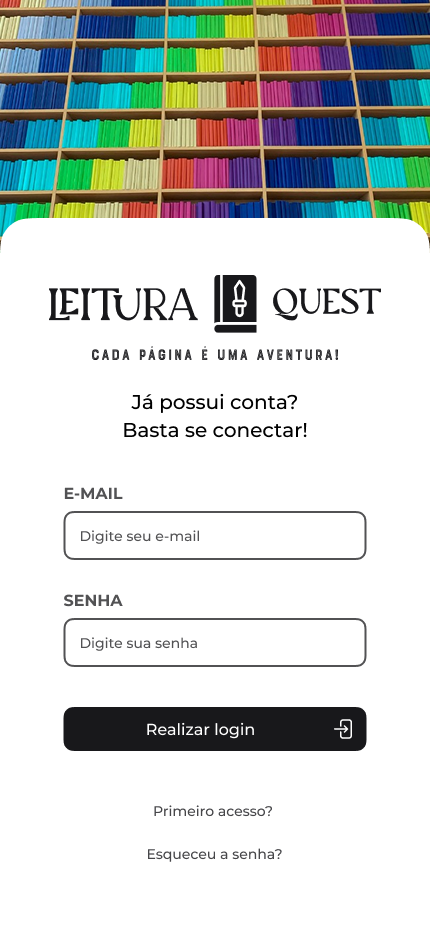
\includegraphics[height=0.58\textheight,keepaspectratio]{../prototipo/images/Login-page.png}
\\[-0.05cm]
\scriptsize Login

\column{0.49\linewidth}
\centering
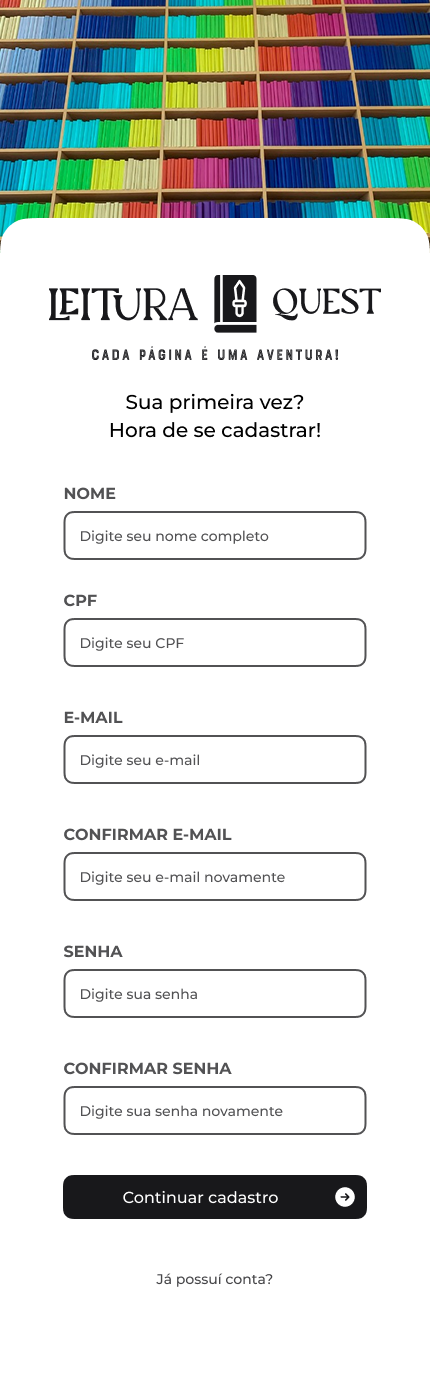
\includegraphics[height=0.58\textheight,keepaspectratio]{../prototipo/images/Register-page-1.png}
\\[-0.05cm]
\scriptsize Cadastro
\end{columns}

\column{0.48\textwidth}
\footnotesize
\textbf{Cobertura funcional}
\begin{itemize}
    \item RF001, RF002, RF017
    \item HU01, HU02, HU03, HU08
    \item Épico EP001 (com conexão a EP003)
\end{itemize}

\textbf{Fluxo observado}
\begin{itemize}
    \item Login por e-mail e senha
    \item Cadastro por etapas
    \item Recuperação de acesso prevista no fluxo
\end{itemize}

\textbf{Dados acionados}
\begin{itemize}
    \item Usuário, Credencial
    \item PreferênciaGênero
    \item Tokens de recuperação de senha
\end{itemize}
\end{columns}
\end{frame}

\begin{frame}{Biblioteca e Leitura (EP003)}
\begin{columns}
\column{0.50\textwidth}
\begin{columns}[T,totalwidth=\linewidth]
\column{0.49\linewidth}
\centering
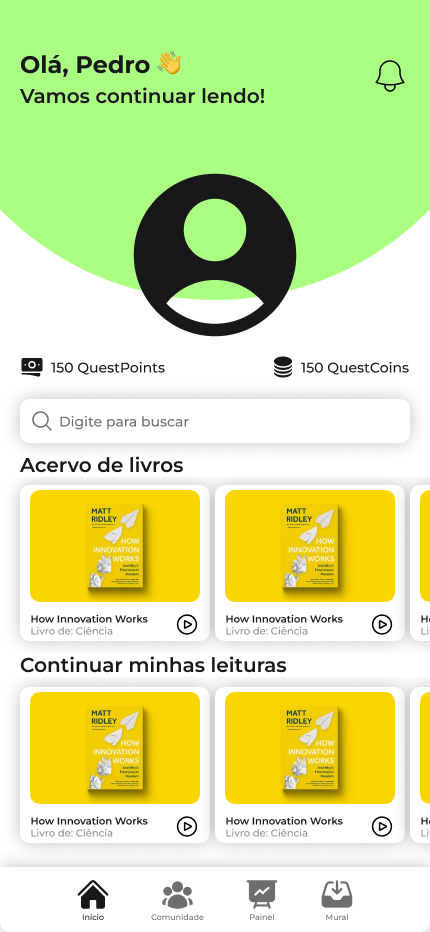
\includegraphics[height=0.58\textheight,keepaspectratio]{../prototipo/images/Home-page.png}
\\[-0.05cm]
\scriptsize Home

\column{0.49\linewidth}
\centering
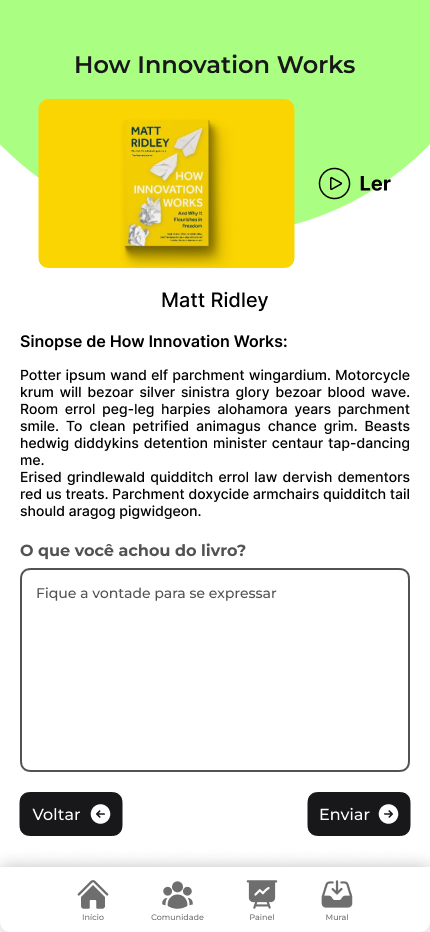
\includegraphics[height=0.58\textheight,keepaspectratio]{../prototipo/images/book-detail-page.png}
\\[-0.05cm]
\scriptsize Detalhe do Livro
\end{columns}

\column{0.48\textwidth}
\footnotesize
\textbf{Cobertura funcional}
\begin{itemize}
    \item RF004, RF005, RF006, RF015, RF016
    \item HU06, HU07
    \item Épico EP003
\end{itemize}

\textbf{Fluxo observado}
\begin{itemize}
    \item Acervo e busca de livros
    \item Sinopse e metadados do livro
    \item Continuidade e progresso de leitura
\end{itemize}

\textbf{Dados acionados}
\begin{itemize}
    \item Livro, Autor, Gênero
    \item Leitura, HistóricoLeitura
    \item Indicadores de progresso por usuário
\end{itemize}
\end{columns}
\end{frame}

\begin{frame}{Gamificação e Perfil (EP002 + EP004)}
\begin{columns}
\column{0.50\textwidth}
\begin{columns}[T,totalwidth=\linewidth]
\column{0.49\linewidth}
\centering
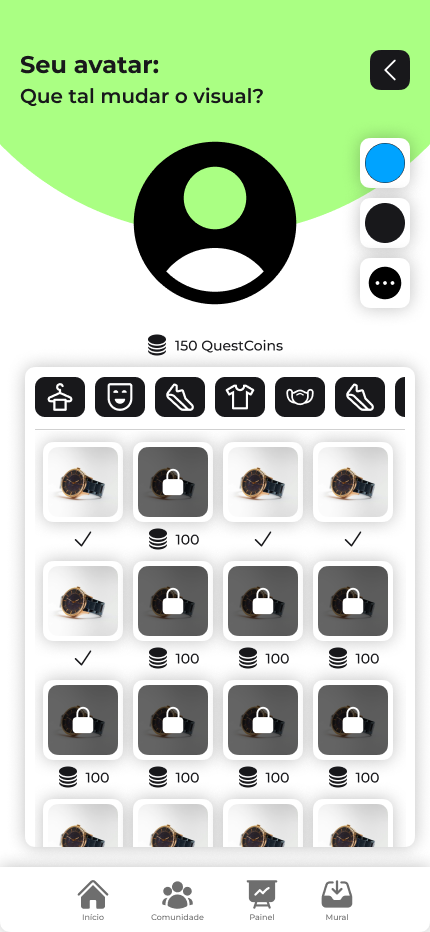
\includegraphics[height=0.58\textheight,keepaspectratio]{../prototipo/images/Store-page.png}
\\[-0.05cm]
\scriptsize Loja

\column{0.49\linewidth}
\centering
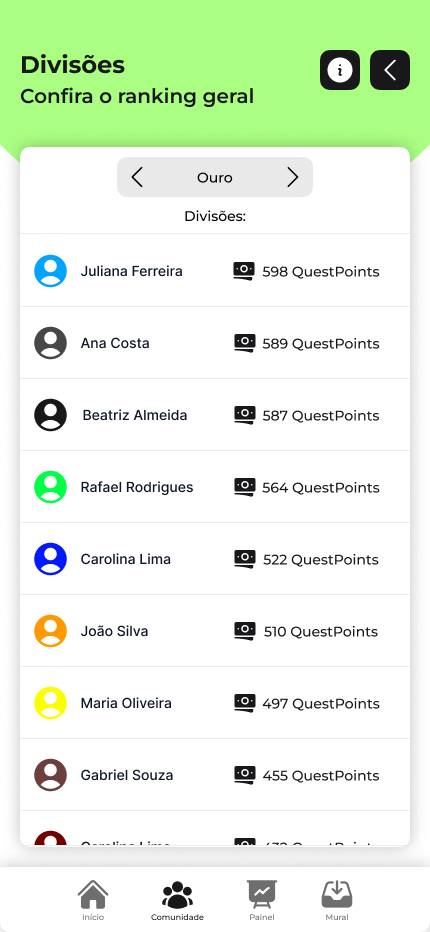
\includegraphics[height=0.58\textheight,keepaspectratio]{../prototipo/images/Ranking-page.png}
\\[-0.05cm]
\scriptsize Ranking
\end{columns}

\column{0.48\textwidth}
\footnotesize
\textbf{Cobertura funcional}
\begin{itemize}
    \item RF003, RF007, RF008, RF018
    \item HU04, HU05, HU09, HU10
    \item Épicos EP002 e EP004
\end{itemize}

\textbf{Fluxo observado}
\begin{itemize}
    \item Loja de itens para avatar
    \item Economia com pontos/moedas
    \item Ranking por divisão e pontuação
\end{itemize}

\textbf{Dados acionados}
\begin{itemize}
    \item Avatar, ItemAvatar, Inventario
    \item SaldoMoedas, Pontuação
    \item Divisão e PosiçãoAluno
\end{itemize}
\end{columns}
\end{frame}

\begin{frame}{Comunidades (EP004 + EP005 + EP007)}
\begin{columns}
\column{0.50\textwidth}
\begin{columns}[T,totalwidth=\linewidth]
\column{0.49\linewidth}
\centering
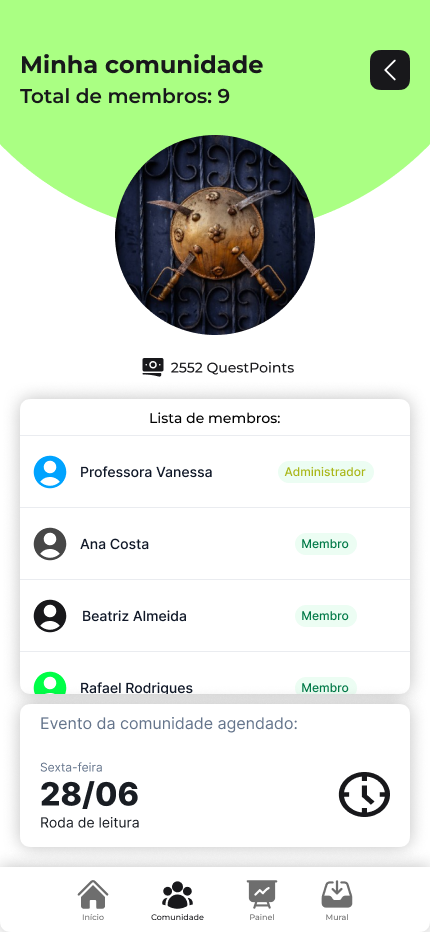
\includegraphics[height=0.55\textheight,keepaspectratio]{../prototipo/images/My-community-page.png}
\\[-0.05cm]
\scriptsize Minha Comunidade

\column{0.49\linewidth}
\centering
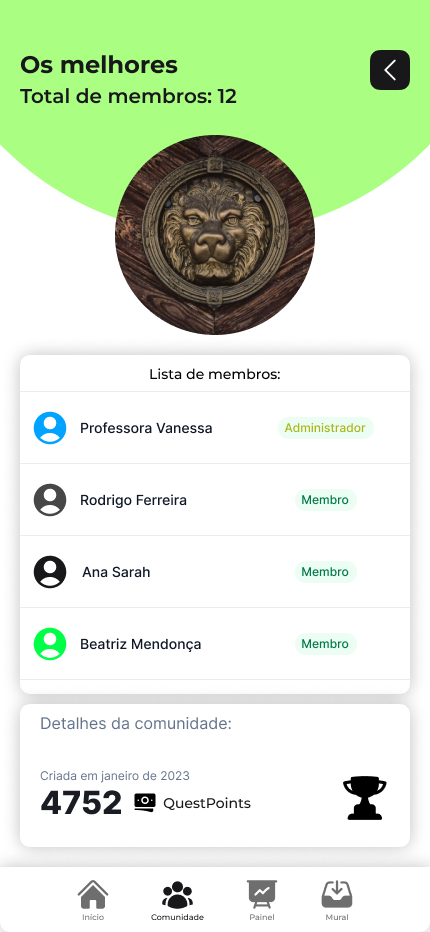
\includegraphics[height=0.55\textheight,keepaspectratio]{../prototipo/images/Other-community-page.png}
\\[-0.05cm]
\scriptsize Outra Comunidade
\end{columns}

\column{0.48\textwidth}
\scriptsize
\textbf{Cobertura funcional}
\begin{itemize}
    \item RF008, RF009, RF010
    \item HU10, HU11, HU15
    \item Épicos EP004, EP005 e EP007
\end{itemize}

\textbf{Fluxo observado}
\begin{itemize}
    \item Visualização de membros, pontuação e organização
    \item Pontuação da comunidade conectada às divisões no ranking geral
    \item Navegação entre comunidade do aluno e outras comunidades
    \item Exposição de evento associado à comunidade
\end{itemize}

\textbf{Dados acionados}
\begin{itemize}
    \item Comunidade, MembroComunidade, Evento
    \item PontuaçãoComunidade, ParticipaçãoAluno
    \item Vínculo com aluno e administrador
\end{itemize}
\end{columns}
\end{frame}

\begin{frame}{Painel, Mural e Avisos (EP006 + EP007)}
\begin{columns}
\column{0.50\textwidth}
\begin{columns}[T,totalwidth=\linewidth]
\column{0.49\linewidth}
\centering
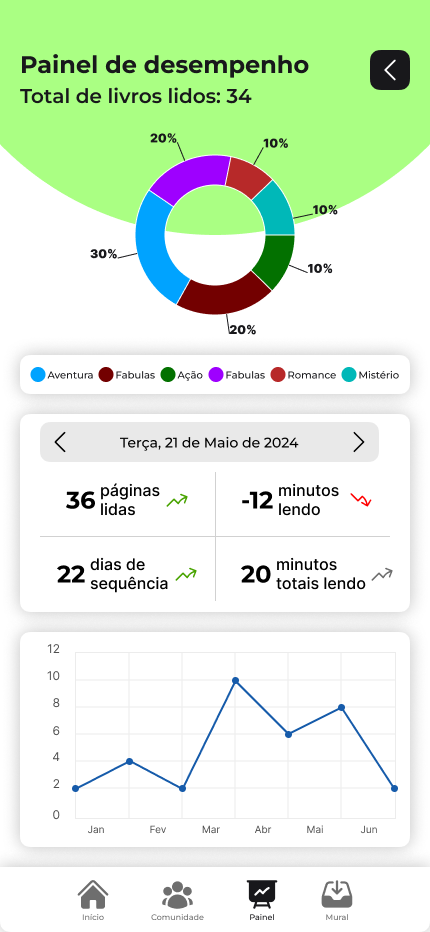
\includegraphics[height=0.58\textheight,keepaspectratio]{../prototipo/images/Panel-page.png}
\\[-0.05cm]
\scriptsize Painel

\column{0.49\linewidth}
\centering
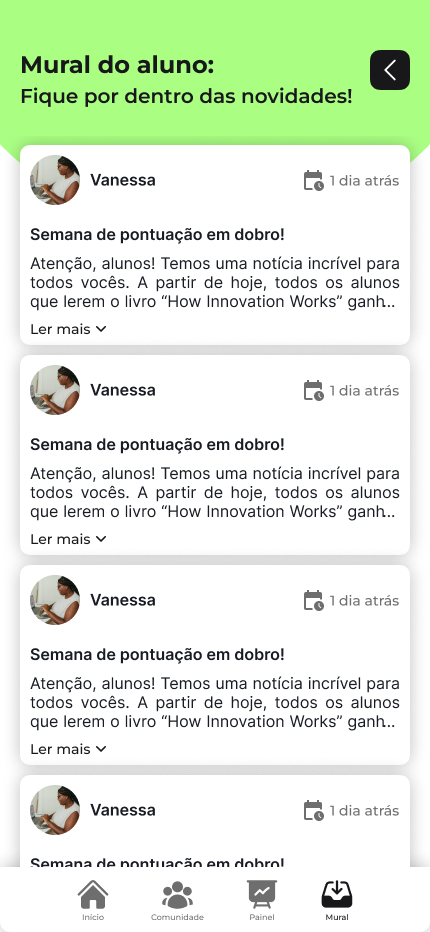
\includegraphics[height=0.58\textheight,keepaspectratio]{../prototipo/images/Mural-page.png}
\\[-0.05cm]
\scriptsize Mural de Avisos
\end{columns}

\column{0.48\textwidth}
\footnotesize
\textbf{Cobertura funcional}
\begin{itemize}
    \item RF012, RF013, RF014, RF018
    \item HU05, HU13, HU16
    \item Épicos EP006 e EP007
\end{itemize}

\textbf{Fluxo observado}
\begin{itemize}
    \item Painel com métricas e evolução do aluno
    \item Exibição cronológica de comunicados
    \item Leitura de título, autoria, data e resumo
    \item Comunicação direta com turmas
\end{itemize}

\textbf{Dados acionados}
\begin{itemize}
    \item MétricaDesempenho, Turma, PerfilAluno
    \item Aviso, Professor, Turma
    \item DataPublicação, ConteúdoResumo
\end{itemize}
\end{columns}
\end{frame}

\section{Relação com Dados}

\begin{frame}{Entidades de Dados Derivadas do Protótipo}
\scriptsize
\begin{tabular}{p{0.27\linewidth} p{0.30\linewidth} p{0.35\linewidth}}
\toprule
\textbf{Tela do protótipo} & \textbf{Dados principais} & \textbf{RFs sustentados} \\
\midrule
Login/Cadastro & Usuário, Credencial, PreferênciaGênero & RF001, RF002, RF017 \\
Home/Detalhe do Livro & Livro, Autor, Gênero, Leitura, HistóricoLeitura & RF004, RF005, RF006, RF015, RF016 \\
Loja/Produto & Avatar, ItemAvatar, Inventario, SaldoMoedas & RF003, RF007 \\
Ranking & Pontuação, Divisão, Temporada, PosiçãoAluno & RF007, RF008 \\
Comunidade & Comunidade, MembroComunidade, Evento & RF009, RF010 \\
Painel/Mural & MétricaDesempenho, Turma, Aviso, Professor & RF012, RF013, RF014, RF018 \\
\bottomrule
\end{tabular}
\end{frame}

\begin{frame}{Conexão com Modelagem de Dados}
\begin{columns}
\column{0.49\textwidth}
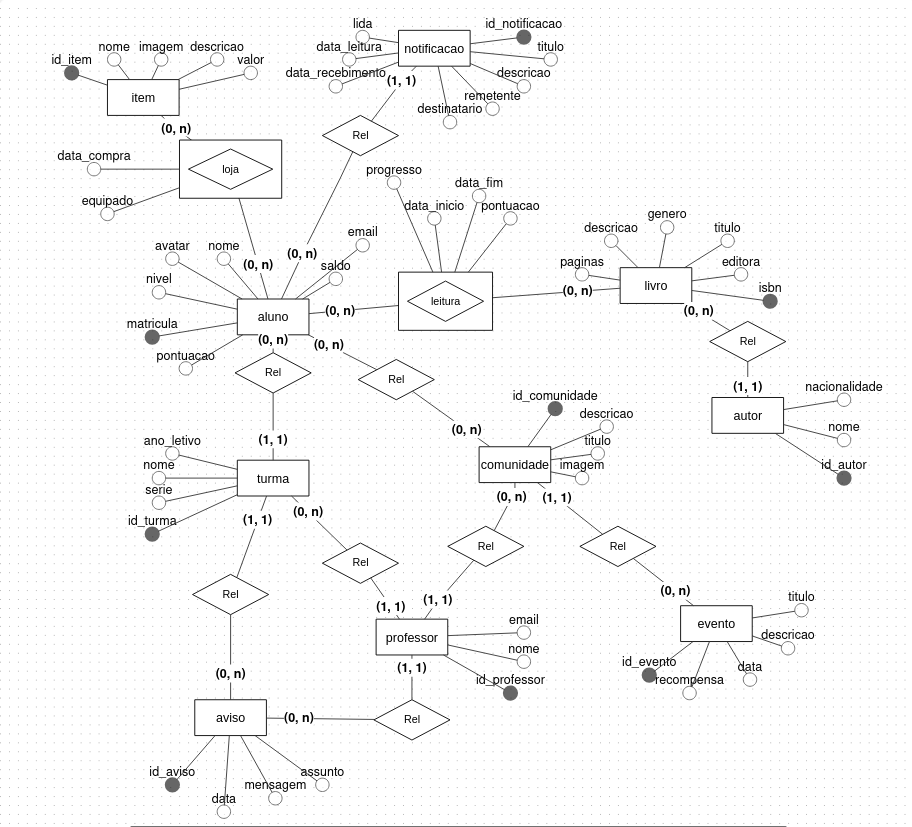
\includegraphics[height=0.42\textheight,keepaspectratio]{../../images/modelo-conceitual-brmodeloweb2.png}
\centering
\scriptsize Modelo Conceitual

\column{0.49\textwidth}
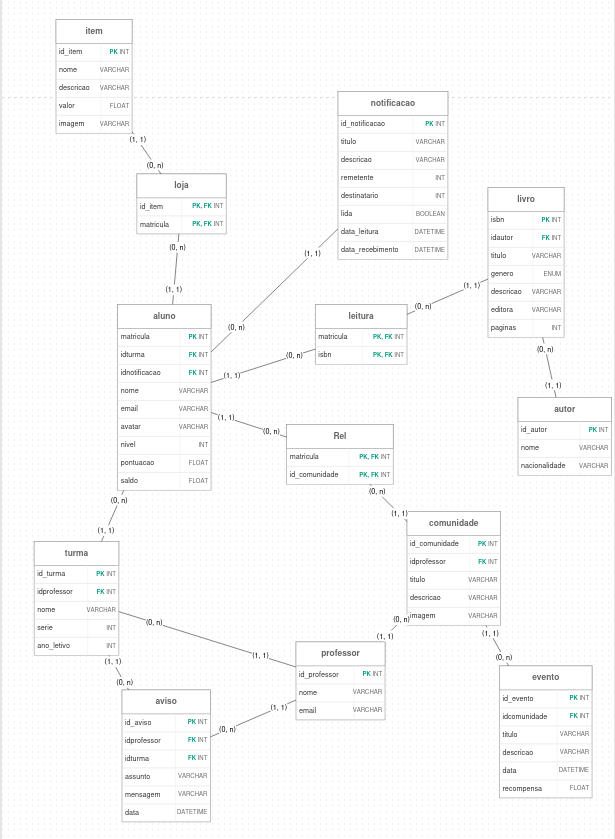
\includegraphics[height=0.42\textheight,keepaspectratio]{../../images/modelo-logico-brmodeloweb2.png}
\centering
\scriptsize Modelo Lógico
\end{columns}

\vspace{0.2cm}
\small
As telas do protótipo antecipam relacionamentos centrais no banco: aluno--leitura, aluno--pontuação,
aluno--comunidade e professor--aviso/evento.
\end{frame}

\begin{frame}{Requisitos Não Funcionais Evidenciados}
\begin{itemize}
    \item \textbf{RNF001 e RNF007:} navegação simples, componentes visuais claros e padrão consistente.
    \item \textbf{RNF003 e RNF009:} estrutura de cards e painéis adequada a diferentes resoluções e navegadores.
    \item \textbf{RNF004 e RNF010:} fluxos de autenticação e recuperação indicam controle de identidade e integridade.
    \item \textbf{RNF002 e RNF006:} ranking, mural e painel reforçam necessidade de consultas eficientes para múltiplos usuários.
\end{itemize}
\end{frame}

\begin{frame}
\Large{\centerline{Obrigado!}}
\end{frame}

\end{document}
